\newpage
\section{Vote Delegation (On-Chain)}
\label{sect:delegation}

All ada holders will have on-chain voting rights, in direct proportion to the exact integral number of lovelace that they hold.
They may delegate these voting rights to any registered delegate, who is expected to act faithfully on their behalf.
Only registered delegates may actually vote on a proposal, but any ada holder may choose to register as a delegate if they choose to do so.
They may then allocate their own vote as they wish, as well as that of any other ada holder who delegates to them.
A delegate may either be an individual or a group that has agreed to act in a specific way.
% \khcomment{There is potentially a transaction cost to voting.  This needs to be considered carefully for acceptability.  Unlike block production, there may be no direct return from voting, so
% this may restrict participation if done wrongly.}\pkcomment{We'll probably need to have a good look at what the researchers have to say on incentives for all the roles}
% \khcomment{Agreed!}
Ada holders may delegate their
vote to any registered delegate by submitting a vote delegation transaction that includes the registered delegate address.
% \khcomment{How do voters know about the available delegates?  They will need to advertise themselves somehow in the voting centre.}
Ada holders may change this delegation at any point in time simply by submitting a new vote delegation transaction.  When votes are tallied, the most recent delegation choice that has been made \emph{prior to the deadline} by each ada holder is considered to be the effective delegation.

\subsection{Delegate Address Registration/De-Registration}
\label{sect:registration}

Delegates must register themselves on-chain.
A deposit is taken when a delegate registers.  Delegates may choose to de-register at any time by submitting a de-registration transaction.  The de-registration takes effect
at the specified future time (which is always an epoch boundary).  Protocol parameters govern the least and greatest notice that must be given for de-registration.  When a delegate de-registers, their deposit is returned,
the address becomes void, and any vote delegation to that address is no longer considered when calculating votes or thresholds.  This means that votes cannot be allocated for a future proposal, and the delegate then
retire but have their vote counted.

\paragraph{Delegate Keys.} Potential delegates must generate a secure key. The following elements are required.

\begin{center}
\begin{tabular}{||l|p{3in}|l||}
  \hline\hline
  \\\hline
  \hline
\end{tabular}
\end{center}
\khcomment{Determine what's required here.}

\paragraph{Registration Certificate.} The delegate registration certificate must include:

\begin{center}
\begin{tabular}{||l|p{3in}|l||}
  \hline\hline
  Delegate public key hash\khcomment{The delegate key structure needs to be confirmed}  & Unique identifier & 32 bytes
  \\\hline
  \hline
\end{tabular}
\end{center}

%% Remove the note about the witness.
% A witness is required for the delegate key. \khcomment{Confirm.}\pkcomment{I don't think so; we do not require a witness for stake address registration, and this should be similar}
The registration comes into effect as soon as the transaction is accepted on-chain.
\khcomment{We could ask for pledge here, but this sounds a bit like vote buying?}

\paragraph{De-Registration Certificate.} Delegate de-registration certificates must include:

\begin{center}
\begin{tabular}{||l|p{3in}|l||}
  \hline\hline
  Delegate public key hash & Unique identifier & 32 bytes
  \\\hline
  Retirement Date & A future epoch & 28 bytes
  \\\hline
  \hline
\end{tabular}
\end{center}

A witness is required for the delegate key. % \khcomment{Confirm this.} Confirmed.

De-registration takes effect from the retirement date (at a specific epoch boundary that may be no sooner than the end of the current epoch, and no more than \emph{maxDelegateRetire} epochs in the future.\khcomment{This needs to be defined, and the size confirmed above.}  Retirement on an epoch boundary ensures that stakeholders do not mistakenly delegate their vote to delegates that will retire before the end of the current epoch.
Vote delegations to a retired delegate are treated in the same way as those to delegates that choose not to vote on a specific issue.

\subsection{Vote Delegation}

Ada stakeholders delegate their vote by issuing an on-chain transaction.  As with normal stake delegation, vote delegation may be transferred from one delegate to another, but can never be retracted.\khcomment{There is an argument that you should  be able to delegate to no-one, but it seems sensible to maintain consistency with the stake delegation mechanism.}

Vote delegation certificates must include:

\begin{center}
\begin{tabular}{||l|p{3in}|l||}
  \hline\hline
  Vote address & Identifies the stake that is to be delegated  & 32 bytes
  \\\hline
  Delegate address & Unique identifier for the delegate & 32 bytes
  \\\hline
  \hline
\end{tabular}
\end{center}
As with stake delegation, posting a vote delegation certificate requires a witness for the delegating vote address.
% As,source.
There is no corresponding vote delegation revocation certificate. If a user wishes to change their delegation choice to a different delegate (which might be themselves),
they can simply post a new delegation certificate. The delegation certificate is revoked automatically when the source vote address is de-registered.

Vote delegation comes into effect immediately that the transaction has appeared on-chain.  % There is no stability window.
Vote delegations may be made at any time up to the point where votes are tallied.
Only vote that is associated with stake in the relevant stake snapshot counts for voting and thresholds.

\paragraph{Voting Centre Requirements}

If they choose to delegate, voters must be able to determine who should receive their vote delegation.  Information should be presented through a voting centre that might include:
\begin{itemize}
\item
Details of the delegate, e.g. their name (which could be the name of a collective group);
\item
Details of the delegate's policies o
\item
Details of the voting record for the delegate (which proposals have been voted for/against and which have not been voted on);
\end{itemize}
See Appendix~\ref{sect:voting-centre}.

\subsection{Vote Addresses}

The Shelley ledger design separates the mechanisms that are used to spend ada from those that are used for block production delegation, embedding two items within a Shelley payment address.

%\begin{figure}[h!]
\begin{center}
  \begin{tabular}{||l|l||}
  \hline\hline
  Payment credential & spending and withdrawal rights \\\hline
  Stake address & block production delegation rights \\\hline
  \hline
  \end{tabular}
\end{center}
%  \caption{Address and key rights in Cardano: Status Quo}
%\end{figure}

The Voltaire design adds an additional item for vote delegatation.

% \begin{figure}[h!]
\begin{center}
  \begin{tabular}{||l|l||}
  \hline\hline
  Payment credential & spending and withdrawal rights (Byron/Shelley) \\\hline
  Stake address & block production delegation rights (Shelley) \\\hline
  Vote address & vote delegation rights (Voltaire) \\\hline
  \hline
\end{tabular}
\end{center}
%  \caption{Address and key rights in Cardano: New Design}
%\end{figure}

It is necessary to register both block and vote delegation intentions on-chain.  This may be done either in a single transaction or in two separate transactions,
as preferred by the user.  The Voltaire design allows independent delegation of vote and block production rights,
and also allows those rights to be independently passed to third parties if required by issuing them with the corresponding secret keys and addresses for either stake delegation, vote delegation, or both.
%\khcomment{Make sure this is clear and consistent with the current stake key approach.} \khcomment{Confirm that a single transaction can be used.}
The keys can be passed on to another party to allow for transfers of delegation rights, or rights may be revoked and new keys/addresses can be issued.

\begin{figure*}[h]
  \begin{center}
  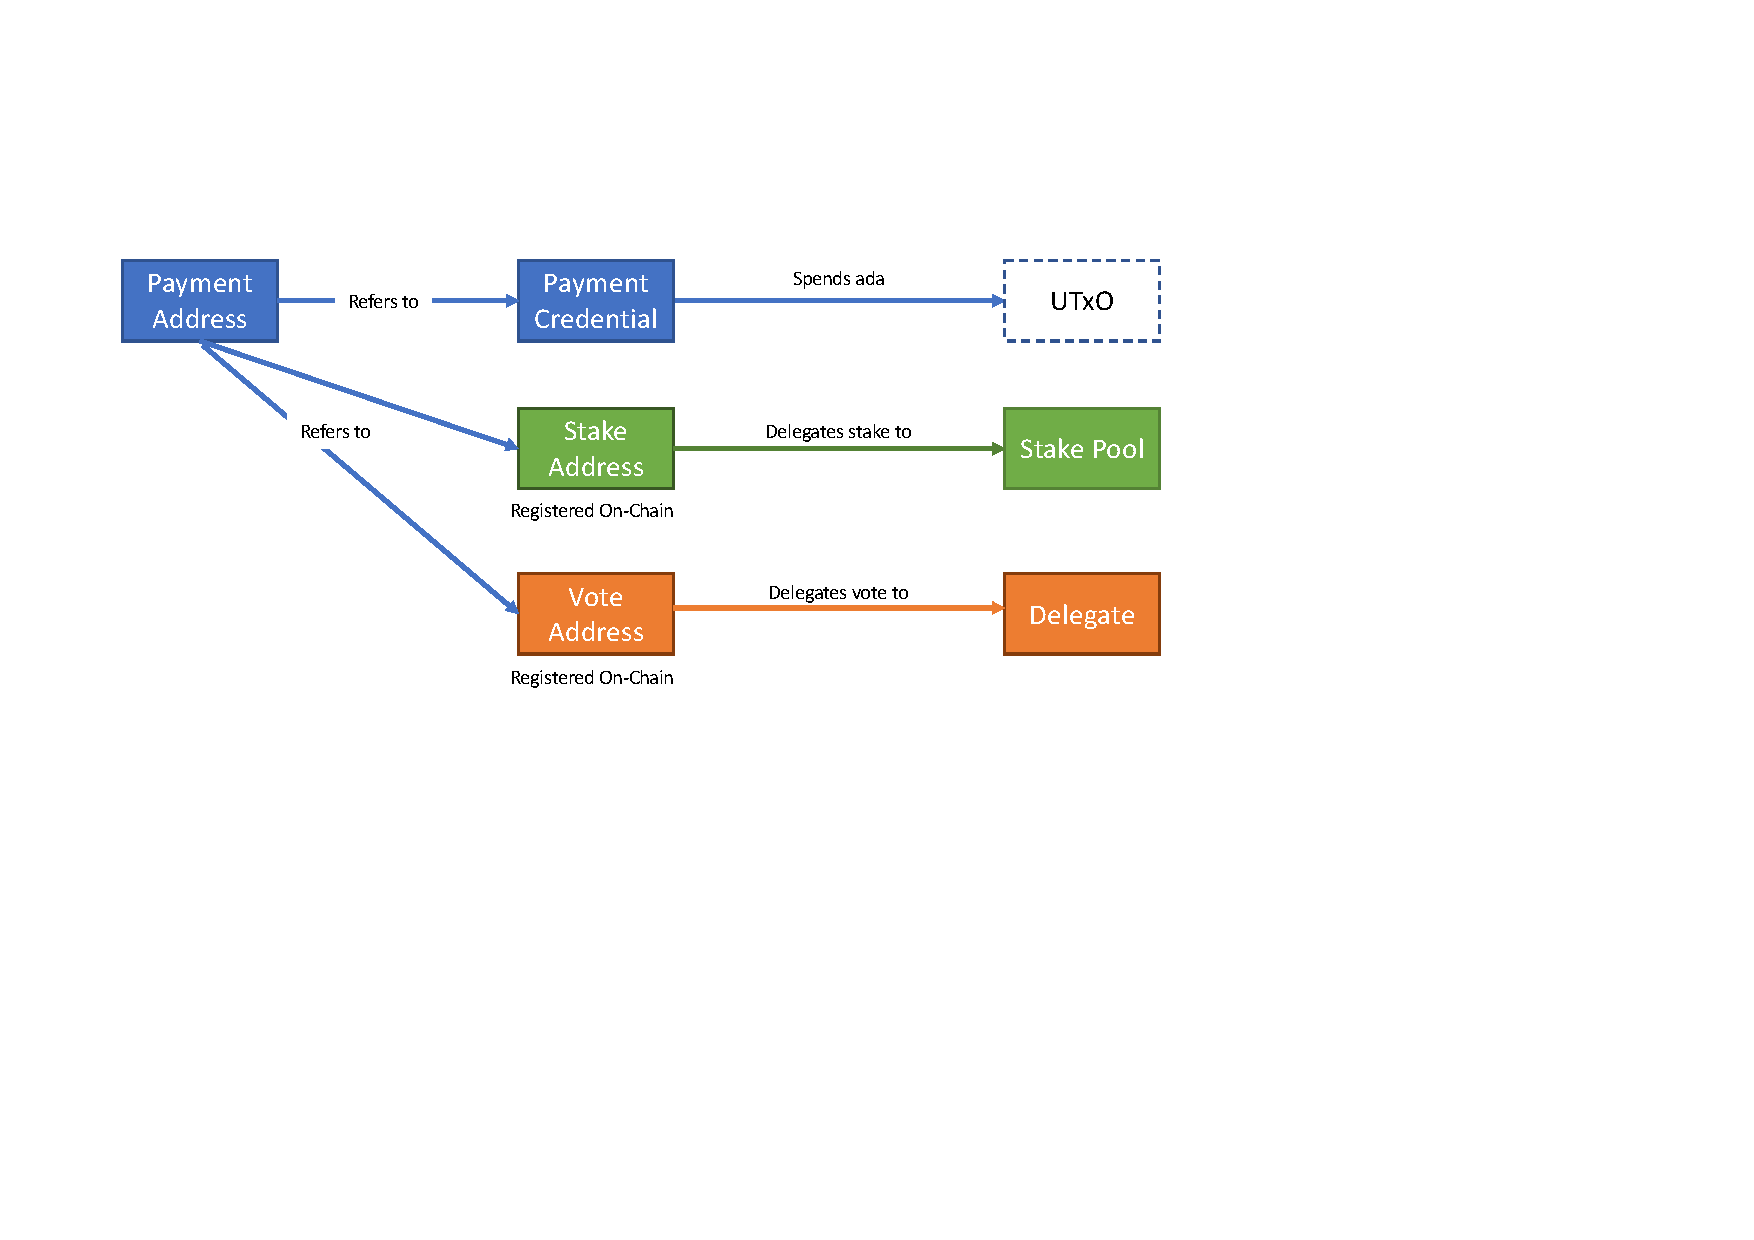
\includegraphics[trim=0 250 150 80,clip,width=\textwidth]{Indirection}
  \end{center}
  \caption{Relationship between payment addresses, payment credentials, vote addresses and stake addresses}
  \label{fig:indirection}
\end{figure*}

\subsubsection*{Payment, Stake and Vote Rights}

Figure~\ref{fig:indirection} outlines how payment addresses relate to payment credentials, stake addresses  and vote addresses.  Payment credentials are used to
authorise payments of any kind, including transacion fees.  Unspent ada is accumulated in UTxOs (Unspent Transaction Outputs).  These UTxOs may either be associated
with the payment address (so returning unspent ada to the user's account), or may be associated with some other address (so allowing ada to be transferred to other wallets,
including those owned by third parties.  If payment credentials are given to a third party, they will have full spending rights over the associated ada.  These rights cannot be
revoked without withdrawing all the associated ada. \khcomment{Not completely clear how the payment address is then removed - there's no on-chain registration.  Does it just become
useless and a target for GC?}
In Shelley, stake addresses are used to delegate block production rights.  They must be registered on chain before use.  They may be passed with the associated secret key to third parties
in order to allow them to delegate on behalf of the ada holder.  This may be useful to protect the original capital while allowing custodial delegation, for example.  Similarly,
the payment credentials may be protected by a hardware wallet, while the stake rights may be protected by software.  This may be more convenient where the hardware wallet is
held securely, for example.
In Voltaire, vote delegation is designed analogously to stake delegation.  It follows that vote rights may be passed on to the same or a different third party (or even retained), as required by the user,
and that voting rights may be asserted without needing the secret payment key.  Both stake and vote addresses may be independently de-registered at any time, in which case the associated delegation rights are immediately
revoked.  New addresses may then be created and assigned as required, and new delegations may be made.  This mechanism also provides protection against lost or stolen stake or vote keys.

\begin{figure*}[h]
  \begin{center}
  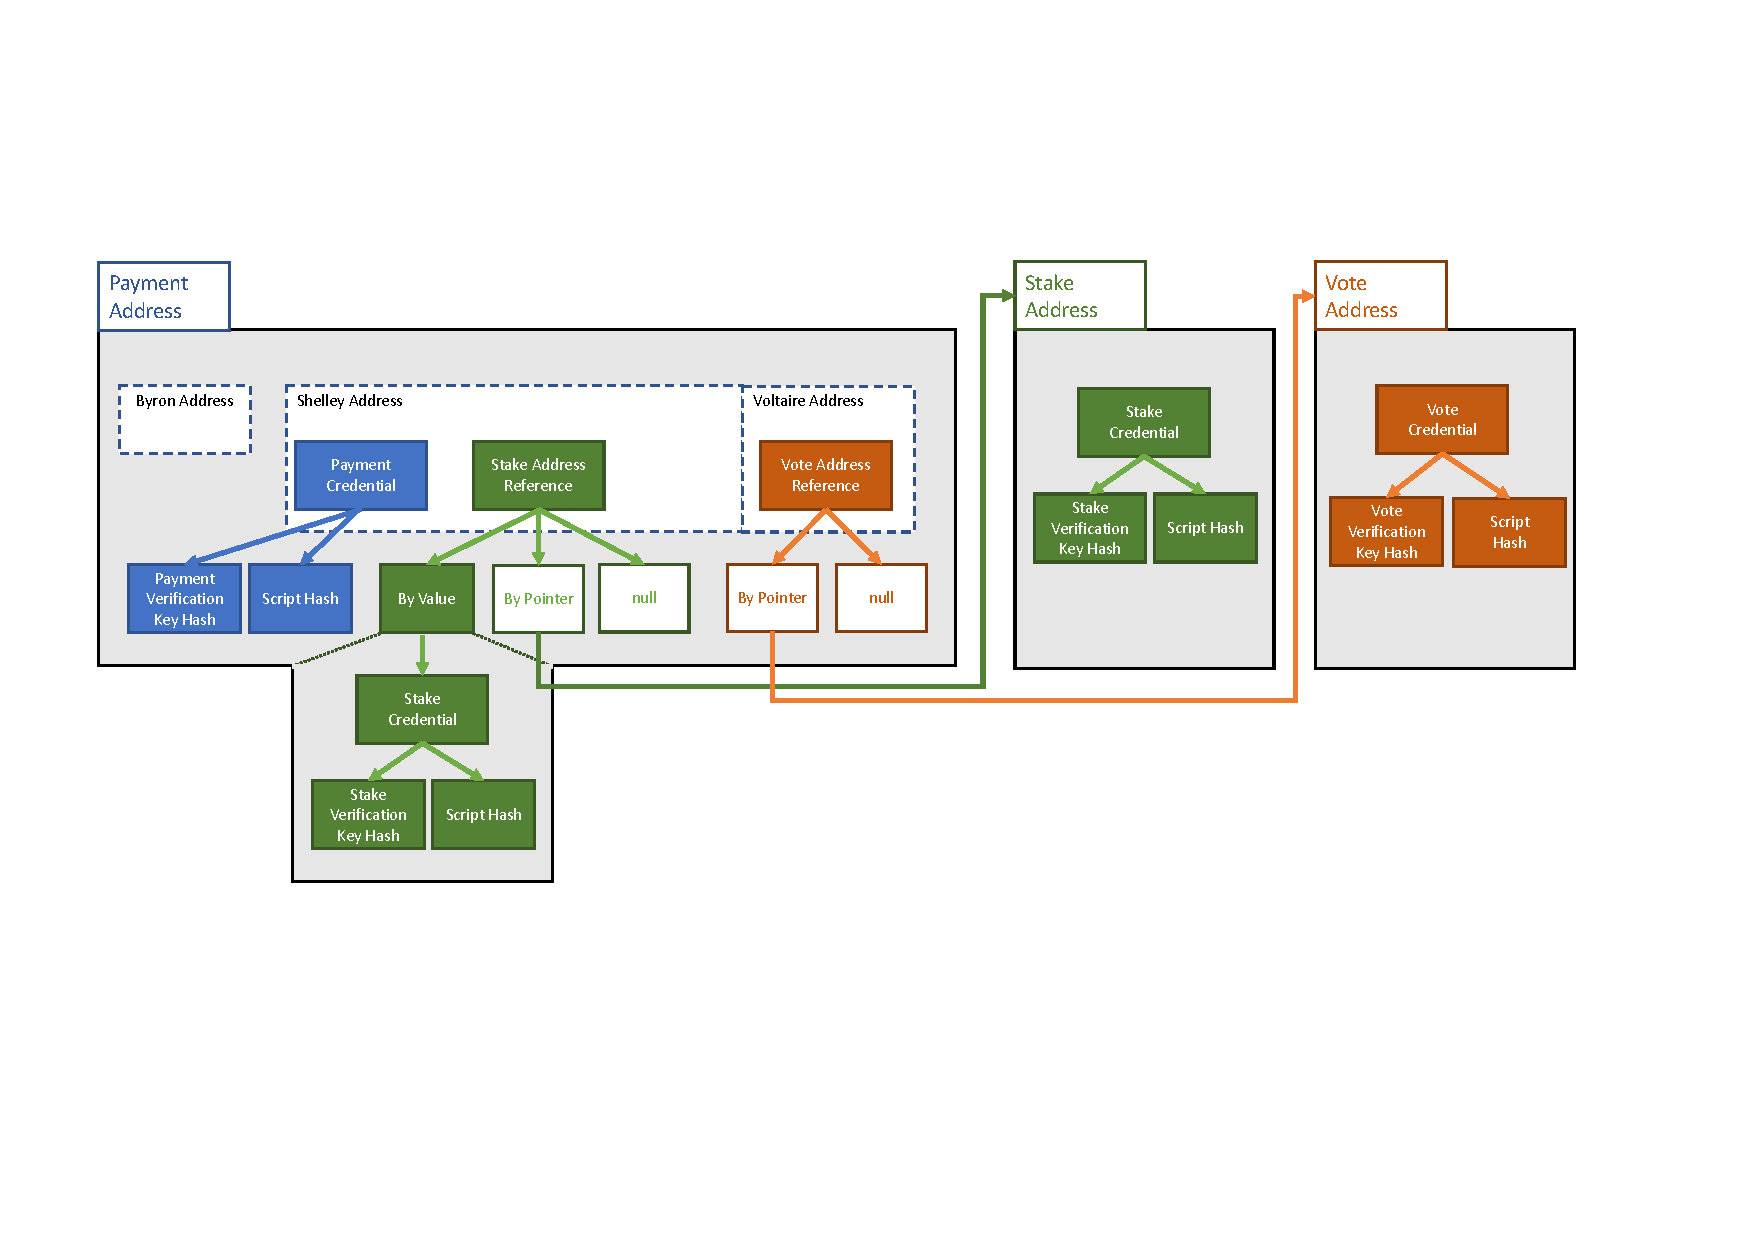
\includegraphics[trim=10 150 30 80,clip,width=\textwidth]{Address-Structure}
  \end{center}
  \caption{Payment Stake and Vote Address Structure}
  \label{fig:address-structure}
\end{figure*}

\subsubsection*{Revised Payment Address Structure}

The revised structure for payment addresses is shown in Figure~\ref{fig:address-structure} (this is adapted from the Shelley delegation design document~\cite{delegation-design}).
Payment addresses may be either Byron Addresses, Shelley Addresses or Voltaire Addresses.
\khcomment{There's apparently no on-chain registration for payment addresses.}
Voltaire addresses extend Shelley addresses by including a vote address reference in addition to the existing payment credential and stake address
reference fields.  Payment credentials may be either payment verification key hashes or script hashes.  Stake address references may be either
by value (in which case the stake credential is directly embedded in the address), by pointer to the registration transaction, or null (an efficient
form used where payment addresses do not need stake delegation rights).
Stake addresses refer to a stake credential that must either be a stake verification key hash or a script hash.
\khcomment{The Shelley address design looks over-complicated -- stake references could probably be collapsed to just pointers.}
Voltaire extends the Shelley address format by including vote address references.  These must be either by pointer to the registration transaction, or null (an efficient
form used where payment addresses do not need vote delegation rights).
\khcomment{I think the null form might not be used?  In which case we could avoid problems by eliminating it.  However, the vote address would then need either to be optional
or it would be necessary to always register the vote credentials with the payment address.}
Vote addresses refer to a vote credential that must be a vote verification key hash.
\khcomment{The different levels seem a bit confusing.  An address is presumably a reference to the structure.  But embedded stake credentials won't have an address.  Credentials similarly
seem to always collapse down to the underlying structure (so may be naming artefects that do not really need to exist).}
\khcomment{Should script hashes be allowed as voting credentials?  I would imagine so.}
The same registration/de-registration concerns apply when pointers are used for vote address references as for stake address references (see ~\cite{delegation-design}).
Although these can be specified separately, enterprise addresses are expected to have both null stake address references and null vote address references.
\khcomment{A single null would do here for both kinds of address reference in an enterprise address, but that would be a bit harder to fit with the existing structure.}

\begin{figure*}[h]
  \begin{center}
  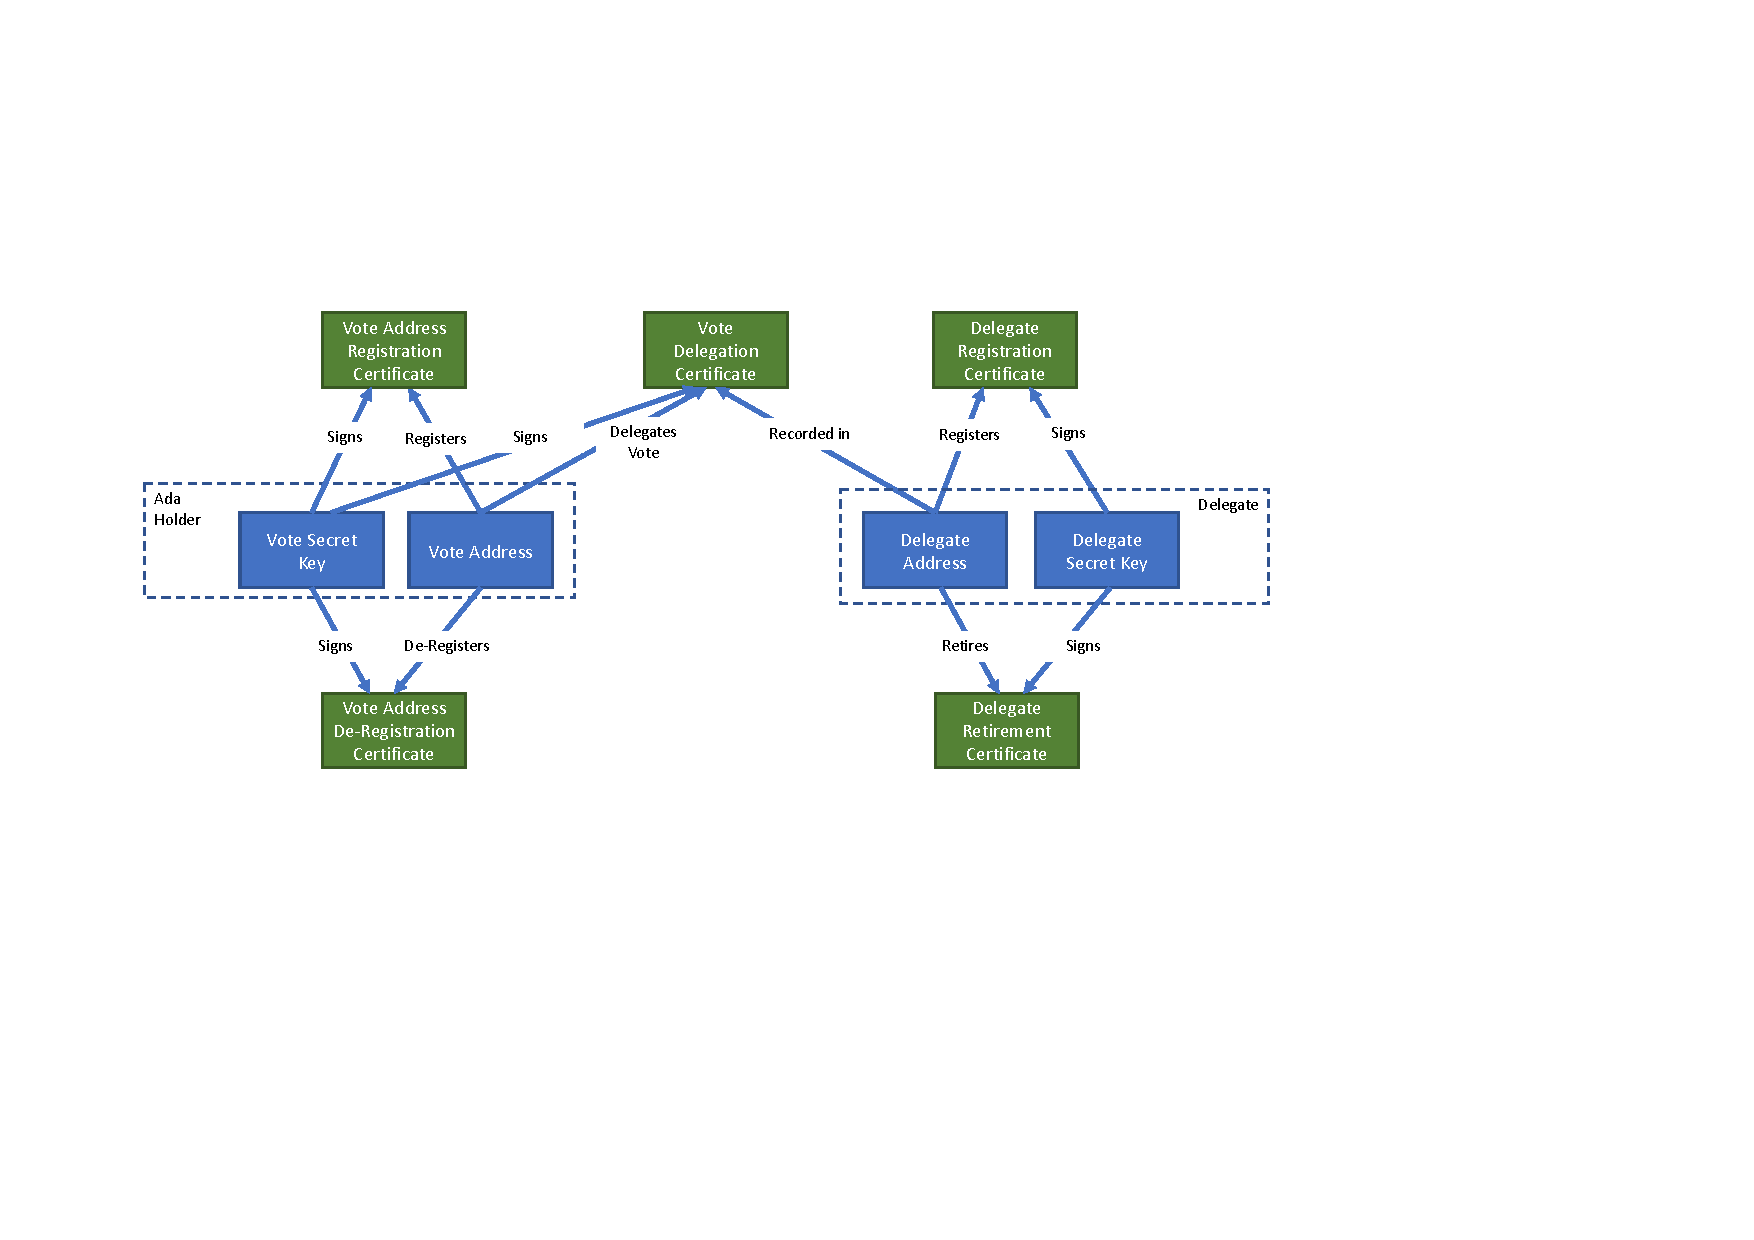
\includegraphics[trim=10 150 30 80,clip,width=\textwidth]{Relationships}
  \end{center}
  \caption{Relationships between vote addresses, keys and certificates}
  \label{fig:relationships}
\end{figure*}

\subsubsection*{Certificates and Registrations}

The Shelley design supports the following kinds of registration certificate to cover the registration/de-registration of stake addresses and stake pools on the blockchain:

\begin{itemize}
\item
Stake address registration certificate;
\item
Stake address de-registration certificate;
\item
Stake delegation certificate;
\item
Stake pool registration certificate;
\item
Stake pool retirement certificate;
\item
Stake pool operational key certificate.
\end{itemize}

The Voltaire design adds the following in an analogous way:

\begin{itemize}
\item
Vote address registration certificate;
\item
Vote address de-registration certificate;
\item
Vote delegation certificate;
\item
Delegate registration certificate;
\item
Delegate retirement certificate;
\end{itemize}



The relationships between these certificates and the vote address and vote keys is shown in Figure~\ref{fig:relationships}.
This is analogous to the design for stake addresses and certificates.
\khcomment{The actual relationships between keys, addresses and certificates are rather unclear in the stake delegation design document.  I think this is correct
but the original document might need to be fixed up...
It's not quite clear when things should be public keys and when they need to be addresses, or which things need actually to be included in the certificates.}
However, unlike the Shelley stake delegation design, the vote design does not need a cold/hot (KES) key structure, a VRF key, or an operational certificate.
\khcomment{I assume hot/cold isn't needed, since security is not directly affected, but I may be wrong?  VRF and operational certificates are certainly not needed.}

\subsubsection*{Certificate Precedence and Validity}

The blockchain specifies a strong and verifiabe temporal ordering on events.
Newer vote, vote delegation, and delegate certificates always override older ones.  Certificates remain in force until they are revoked or a newer certificate is issued,
whichever comes first.  Vote and delegate certificates may be revoked.  Vote delegations are not explicitly revoked, but are only valid when both the vote certificate
and delegate certificate are also in force.
Newer delegation certificates override older delegation certificates. This allows delegators to move from one stake pool to another.
